\documentclass{article}
\usepackage{graphicx} % Required for inserting images
\usepackage{float}
\usepackage{amsmath}
\usepackage{hyperref}

\graphicspath{{images}}

\title{Programming Project 2}
\author{Giorgio Bertone, Jura Hostic}
\date{December 2024}


\begin{document}

\maketitle

\section{Task 1}
\subsection{Genetic Algorithm}

The GA framework operates on a population of candidate solutions, represented as permutations of graph vertices $V$, to minimize edge crossing costs while satisfying precedence constraints. The fitness function incorporates a penalty mechanism to discourage constraint violations, and ensure feasible solutions are favored.

\subsubsection*{Parameters}
\begin{itemize}
    \item \textbf{Population Size}: Number of individuals in each generation.
    \item \textbf{Generations}: Total number of generations to evolve.
    \item \textbf{Elite Size}: Number of top individuals preserved unaltered (elitism).
    \item \textbf{Tournament Size}: Size of subsets for tournament-based parent selection.
    \item \textbf{Mutation Rate}: Probability of applying mutation to offspring.
    \item \textbf{Crossover Rate}: Probability of applying the crossover operator.
    \item \textbf{Constraint Penalty}: Penalty weight for constraint violations in fitness evaluation.
\end{itemize}

\subsubsection*{Fitness Function}
The fitness function combines the objective function (computed using \textit{cost\_function\_bit}) and a penalty term proportional to the number of violated constraints to balance minimization of edge crossings with adherence to problem constraints.

\subsubsection*{Genetic Operators}

\begin{enumerate}
    \item \textbf{Selection}: A tournament selection mechanism is used to choose parents, favoring individuals with higher fitness.
    \item \textbf{Crossover}: The Order Crossover (OX) operator generates offspring by preserving subsequences from one parent while maintaining valid permutations.
    \item \textbf{Mutation}: Swap mutation, involving a variable number of element swaps, is applied to introduce diversity.
    \item \textbf{Repair}: A repair mechanism ensures offspring are feasible by adjusting orderings to satisfy constraints when necessary.
\end{enumerate}

\subsubsection*{Algorithm}
\begin{itemize}
    \item \textbf{Initialization}: The initial population is generated randomly and the individuals representing invalid solutions are repaired to ensure feasibility.
    \item \textbf{Evaluation}: Fitness scores are calculated for each individual in the population.
    \item \textbf{Selection and Reproduction}: Parents are selected through tournament selection, and offspring are produced using crossover, mutation, and repair.
    \item \textbf{Elitism}: The best-performing individuals are carried forward unchanged.
    \item \textbf{Iteration}: The process is repeated for a predefined number of generations, recording fitness statistics at each step.
\end{itemize}

\subsection{Ant Colony Optimization}
The MaxMin Ant System (MMAS) is a variation of the ACO metaheuristic, that controls the maximum and minimum pheromone amounts on each trail in order to avoid stagnation. Indeed, it has been shown empirically that MMAS strikes a good balance between intensification (exploiting good solutions) and diversification (exploring new regions). The MWCCP is modeled as a graph optimization problem, where ants traverse the solution space guided by pheromone trails and heuristic information.

\subsubsection*{Parameters}
\begin{itemize}
    \item \textbf{Alpha ($\alpha$)}: Controls the influence of pheromones on ant decision-making; higher values promote exploitation.
    \item \textbf{Beta ($\beta$)}: Controls the importance of heuristic information; higher values favor heuristic-driven exploration.
    \item \textbf{Evaporation Rate ($\rho$)}: Regulates pheromone decay; higher values reduce old pheromone influence more aggressively, enhancing exploration.
    \item \textbf{Ant Count}: Determines the number of ants per iteration; more ants increase diversity, but raise computational cost.
    \item \textbf{Iterations}: Sets the number of algorithm cycles; more iterations allow deeper exploration but require more time.
    \item \textbf{Tau Min ($\tau_{min}$)}: Limits minimum pheromone levels; prevents solution components from being ignored.
    \item \textbf{Tau Max ($\tau_{max}$)}: Caps maximum pheromone levels; ensures search diversity.
\end{itemize}


\subsubsection*{Components}
\begin{itemize}
    \item \textbf{Pheromone Matrix}: Initialized uniformly with high values to encourage exploration in early iterations.
    \item \textbf{Heuristic Information}: Derived from graph properties, such as vertex in-degree or edge weights, to prioritize promising candidates during solution construction.
\end{itemize}

\subsubsection*{Algorithm}
\begin{enumerate}
    \item \textbf{Initialisation}: The pheromone matrix and the heuristic information matrix are created as discussed above
    \item \textbf{Solution Construction}: Each ant constructs an ordering of the vertices probabilistically based on pheromone intensity and heuristic attractiveness of each candidate vertex. The probabilities are calculated as a weighted combination of these factors, controlled by parameters that adjust their influence.
    \item \textbf{Constraints Handling}: After constructing a solution, the algorithm verifies if it satisfies the constraints. If not a a repair mechanism rearranges it.
    \item \textbf{Pheromone Update}: After all ants construct solutions, the pheromone levels are updated based on the global best solution. Evaporation is also applied to ensure pheromone decay over time, preventing premature convergence. Then the pheromone values are clipped.
    \item \textbf{Dynamic Adjustment}: Upper and lower bounds for the pheromone levels are dynamically adjusted based on the best solution cost to maintain diversity and guide the search effectively.
    \item \textbf{Iteration}: The algorithm iterates over multiple cycles, with each cycle involving solution construction, evaluation, and pheromone updates.

\end{enumerate}

\section{Task 2}

\subsection{SMAC3}
For the hyperparameter optimization process we used SMAC3. SMAC3 is an open-source optimization framework design for challenging algorithm configuration and hyperparameter optimization problems.
The framework uses Bayesian Optimization in combination with an aggresive racing mechanism to eficiently deterime which configurations are the best while balancing exploration and exploitation.
The \href{https://jmlr.org/papers/v23/21-0888.html}{research paper} is and the \href{https://github.com/automl/SMAC3}{framework} is available for use.

\subsection{Final Configurations}
The hyperparameter optimizations was done on medium tuning instances for time reasons. Smaller experiments were done on other instances with similar results.
The SMAC3 framework was used.

For evaluating fitness, the algorithms were run on all medium tuning instances and the fitness was calculated using the cumulative cost and time using the following formula:
\[
F =
\begin{cases}
	C \cdot T & \text{if } T \leq 60 \, \text{s}, \\
	\frac{C \cdot T}{60} & \text{if } T > 60 \, \text{s}.
\end{cases}
\]
The formula penalises longer running times which become too long on bigger instances, while considering all configurations with reasonable running times the same time wise to
allow for limiting the comparison to the quality of the solutions. The time cutoff for penalisation was set to 60 seconds from testing the time differences of medium and large instances.

\subsubsection{Genetic Algorithm}
The genetic algorithm parameters was optimized using the following intervals:
\begin{align*}
	\text{Population Size:} & \quad [20, 250] \\
	\text{Generations:} & \quad [10, 250] \\
	\text{Elite Size:} & \quad [0, 20] \\
	\text{Tournament Size:} & \quad [3, 30] \\
	\text{Mutation Rate:} & \quad [0.1, 0.6] \\
	\text{Crossover Rate:} & \quad [0.4, 1] \\
	\text{Constraint Penalty:} & \quad [10{,}000, 1{,}000{,}000]
\end{align*}

The tuning process was run for 250 trials. The best configuration found was:
\begin{align*}
	\text{Population Size:} & \quad 40 \\
	\text{Generations:} & \quad 150 \\
	\text{Elite Size:} & \quad 13 \\
	\text{Tournament Size:} & \quad 25 \\
	\text{Mutation Rate:} & \quad 0.255 \\
	\text{Crossover Rate:} & \quad 0.79 \\
	\text{Constraint Penalty:} & \quad 213178
\end{align*}

\subsubsection{Ant Colony Optimization}
The ant colony optimization parameters was optimized using the following intervals:
\begin{align*}
    \text{Alpha:} & \quad [1.0, 2.0] \\
    \text{Beta:} & \quad [1.0, 2.0] \\
    \text{Evaporation Rate:} & \quad [0.1, 0.9] \\
    \text{Ant Count:} & \quad [20, 100] \\
    \text{Iterations:} & \quad [50, 250] \\
    \text{Tau Min:} & \quad [0.1, 1.0] \\
    \text{Tau Max:} & \quad [1.0, 10.0]
\end{align*}
The tuning process was run for 250 trials. The best configuration found was:
\begin{align*}
    \text{Alpha:} & \quad 1.87 \\
    \text{Beta:} & \quad 1.07 \\
    \text{Evaporation Rate:} & \quad 0.69 \\
    \text{Ant Count:} & \quad 22 \\
    \text{Iterations:} & \quad 55 \\
    \text{Tau Min:} & \quad 0.51 \\
    \text{Tau Max:} & \quad 7.85
\end{align*}

\subsection{Influence of Parameters}
The paramaters which were chosen during the optimization process strike a balance between solution quality and the time required to find it.
The following graphs show the influence of different parameters on the solution quality and the time required to find it.
In most of them, you can see that the parameter value which was chosen during the optimization process (Red dots in graphs) is often one of the best values for the cost and time trade-off.
The graphs are cumulative cost and time over all medium tuning instances, with the parameter values being the same as the ones used in the final configuration except for the parameter being tested.
\subsubsection{Genetic Algorithm}
\begin{figure}[H]
    \centering
    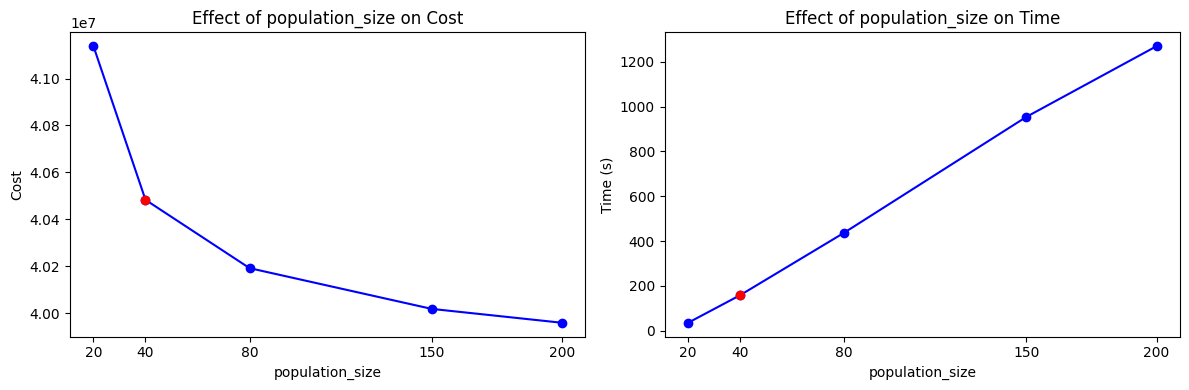
\includegraphics[width=\linewidth]{effect_of_population_size.png}
    \caption{Influence of Population Size on Fitness}
    \label{fig:pop_size}
\end{figure}

\begin{figure}[H]
    \centering
    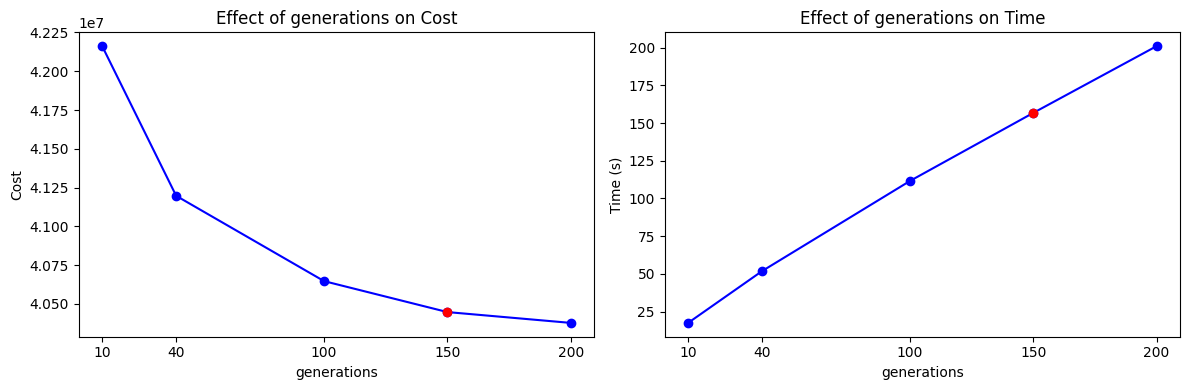
\includegraphics[width=\linewidth]{effect_of_generations.png}
    \caption{Influence of Generations on Fitness}
    \label{fig:generations}
\end{figure}

\begin{figure}[H]
    \centering
    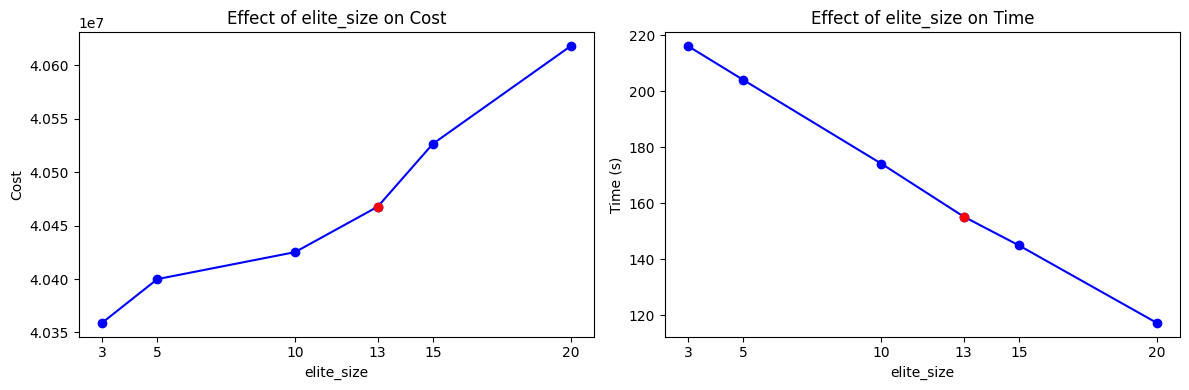
\includegraphics[width=\linewidth]{effect_of_elite_size.png}
    \caption{Influence of Elite Size on Fitness}
    \label{fig:elite_size}
\end{figure}

\begin{figure}[H]
    \centering
    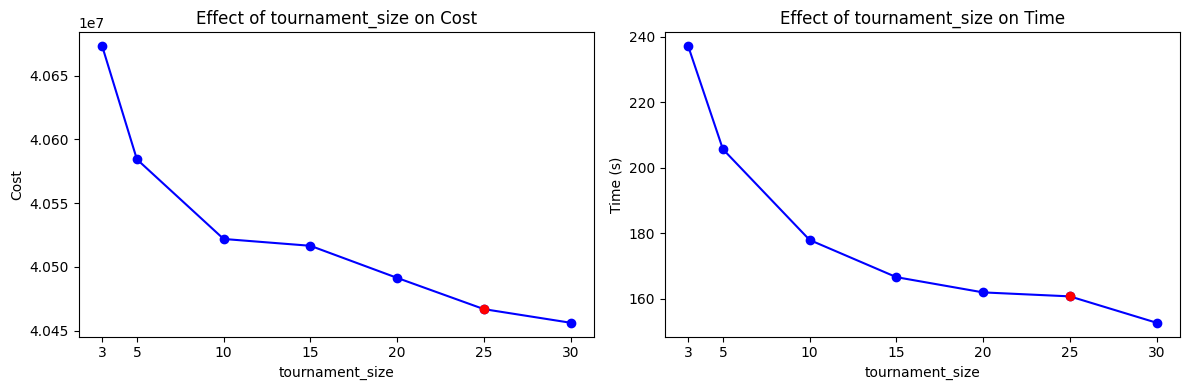
\includegraphics[width=\linewidth]{effect_of_tournament_size.png}
    \caption{Influence of Tournament Size on Fitness}
    \label{fig:tournament_size}
\end{figure}

\begin{figure}[H]
    \centering
    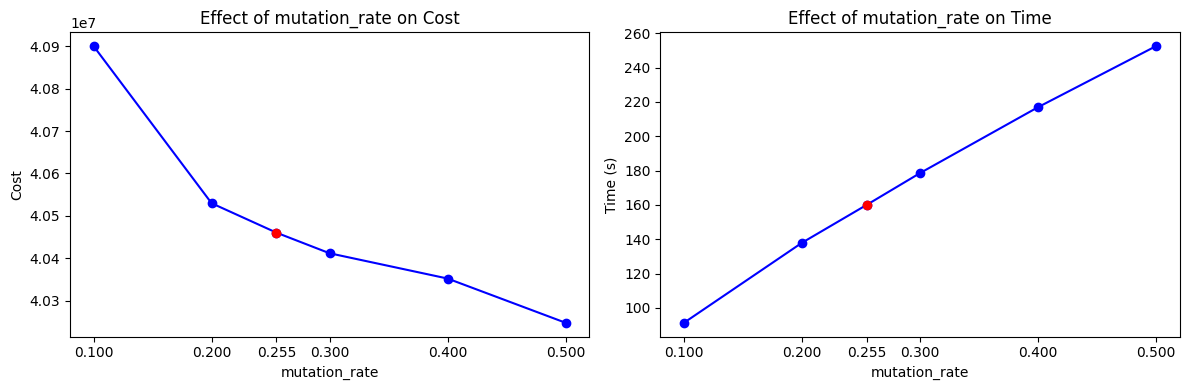
\includegraphics[width=\linewidth]{effect_of_mutation_rate.png}
    \caption{Influence of Mutation Rate on Fitness}
    \label{fig:mutation_rate}
\end{figure}

\begin{figure}[H]
    \centering
    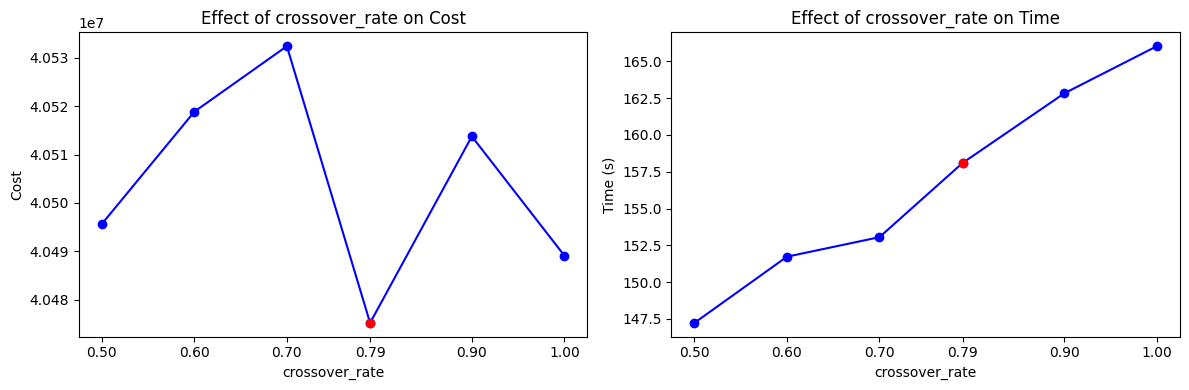
\includegraphics[width=\linewidth]{effect_of_crossover_rate.png}
    \caption{Influence of Crossover Rate on Fitness}
    \label{fig:crossover_rate}
\end{figure}

\begin{figure}[H]
    \centering
    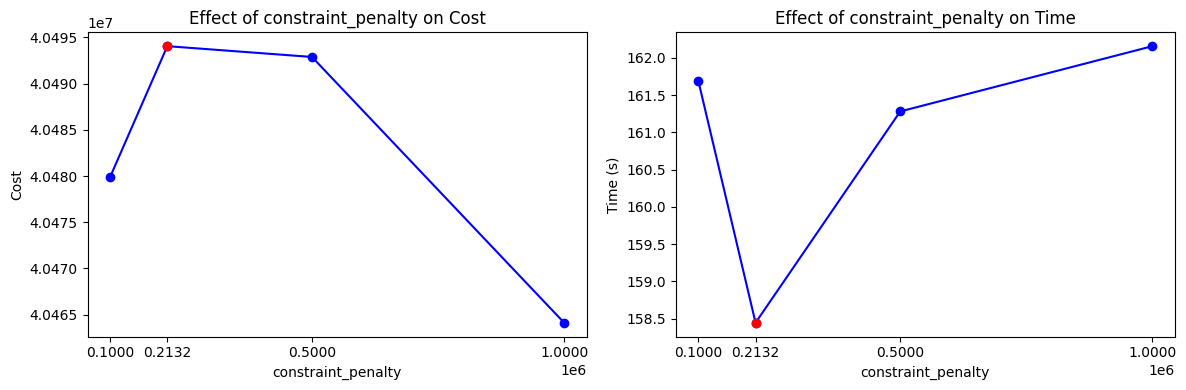
\includegraphics[width=\linewidth]{effect_of_constraint_penalty.png}
    \caption{Influence of Constraint Penalty on Fitness}
    \label{fig:constraint_penalty}
\end{figure}

\subsubsection{Ant Colony Optimization}
\begin{figure}[H]
    \centering
    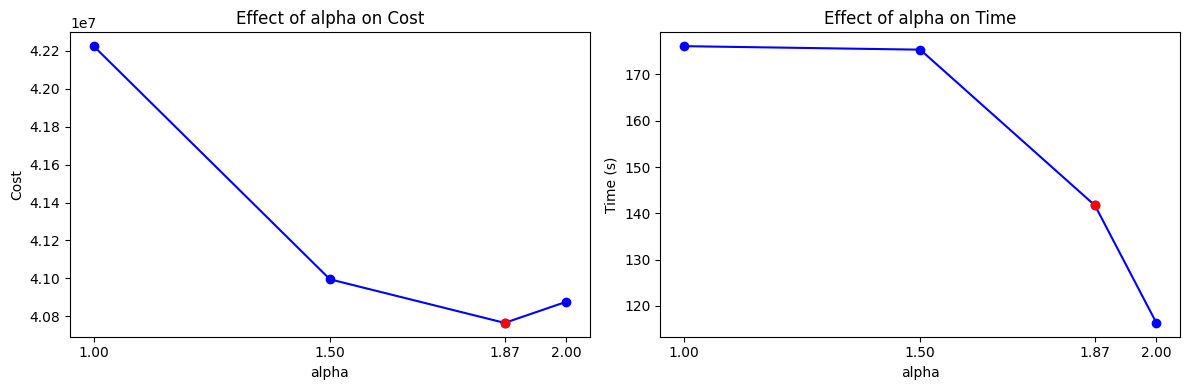
\includegraphics[width=\linewidth]{effect_of_alpha.png}
    \caption{Influence of Alpha on Fitness}
    \label{fig:alpha}
\end{figure}

\begin{figure}[H]
    \centering
    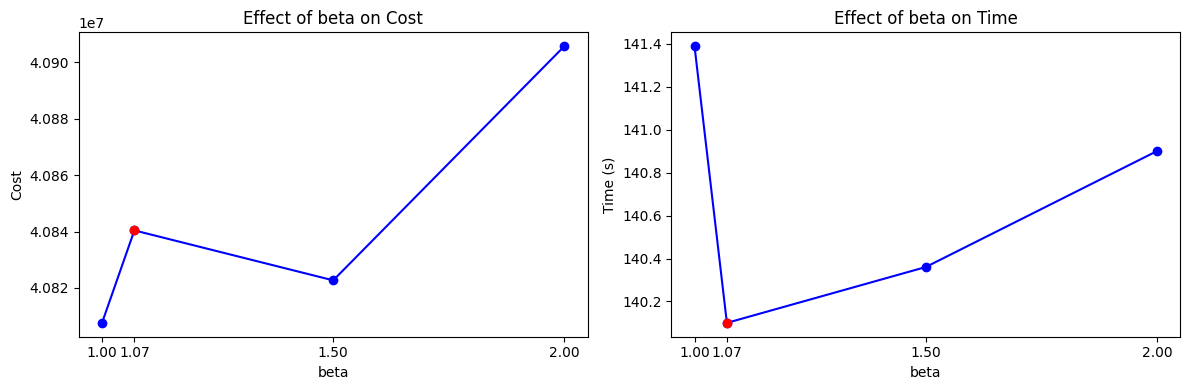
\includegraphics[width=\linewidth]{effect_of_beta.png}
    \caption{Influence of Beta on Fitness}
    \label{fig:beta}
\end{figure}

\begin{figure}[H]
    \centering
    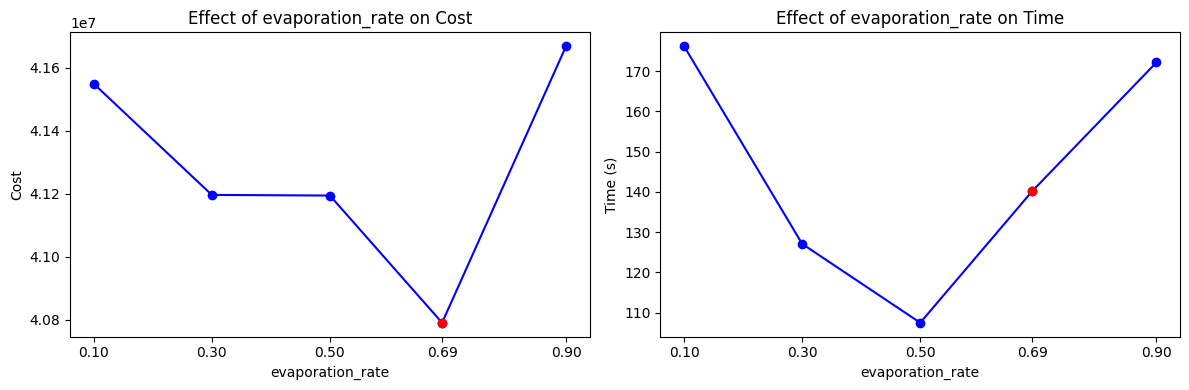
\includegraphics[width=\linewidth]{effect_of_evaporation_rate.png}
    \caption{Influence of Evaporation Rate on Fitness}
    \label{fig:evaporation_rate}
\end{figure}

\begin{figure}[H]
    \centering
    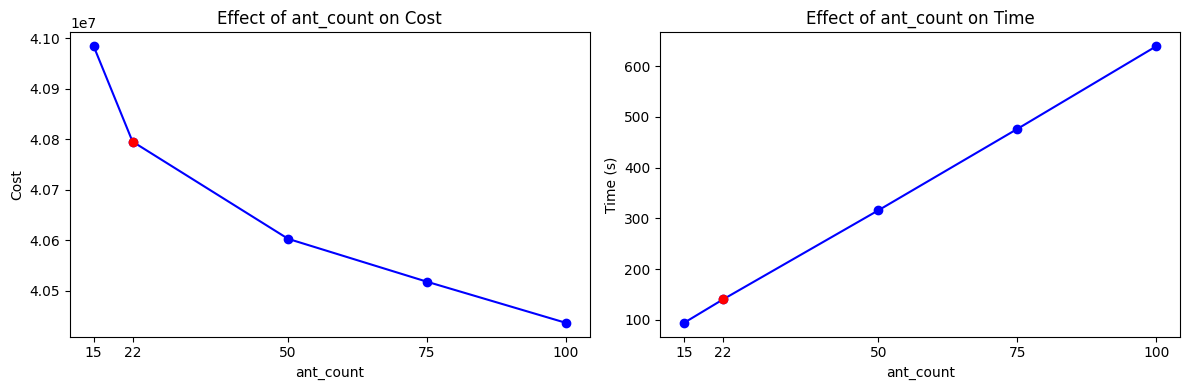
\includegraphics[width=\linewidth]{effect_of_ant_count.png}
    \caption{Influence of Ant Count on Fitness}
    \label{fig:ant_count}
\end{figure}

\begin{figure}[H]
    \centering
    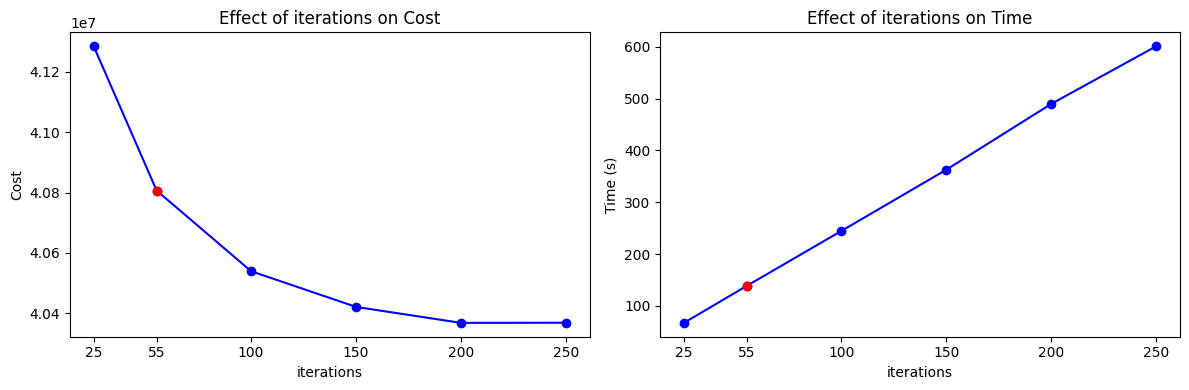
\includegraphics[width=\linewidth]{effect_of_iterations.png}
    \caption{Influence of Iterations on Fitness}
    \label{fig:iterations}
\end{figure}

\begin{figure}[H]
    \centering
    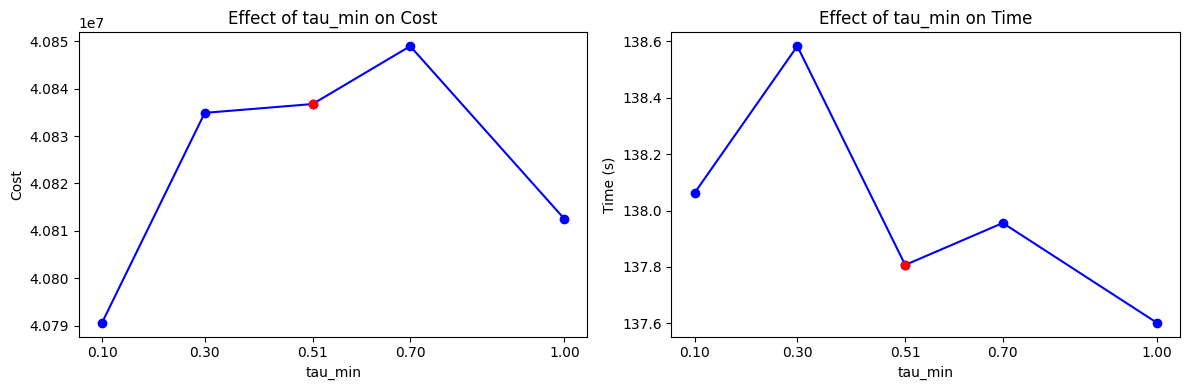
\includegraphics[width=\linewidth]{effect_of_tau_min.png}
    \caption{Influence of Tau Min on Fitness}
    \label{fig:tau_min}
\end{figure}

\begin{figure}[H]
    \centering
    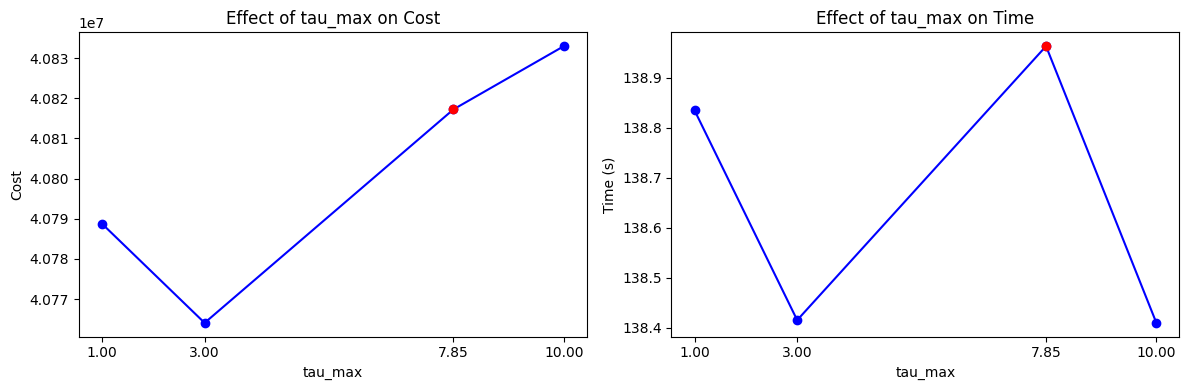
\includegraphics[width=\linewidth]{effect_of_tau_max.png}
    \caption{Influence of Tau Max on Fitness}
    \label{fig:tau_max}
\end{figure}

\subsection{Bottlenecks}

TODO


\section{Task 3}

We now have to test whether there is a significant difference between the performance of the two algorithms on the test instances. To do so, we apply the tuned algorithms several times on each test instance and then get the best performance for each instance. Then compare them using a statistical test for paired samples since the objective function values are determined on the same instances. 
\subsection{Small}
We first test if the difference of both samples is approximately normally distributed.
\begin{figure}[H]
    \centering
    \includegraphics[width=0.5\linewidth]{small_diff.png}
    \caption{Performance difference on small instances}
    \label{fig:enter-label}
\end{figure}
 Since this is not the case we decided to use the \textbf{Wilcoxon-Test}.  We use a two-sided test to test wether there is a significant difference betweeen the two algorithms. The null hypothesis is $$
 H_0 : \theta_{GA} = \theta_{ACO} $$
 and the alternative is
 $$
 H_1 : \theta_{GA} \neq \theta_{ACO}
 $$
 We get: 
 \begin{verbatim}
Test Result: 
p-value = 0.0020 
H0 can be rejected on a level of significance of 0.05 
 \end{verbatim}
 We can reject the null hypothesis which means there is statistical evidence for the two performances to be different.

 To interpret the direction of the effect, since we can not repeat a test changing alternative as this would be considered p-hacking, we now look at the mean and median of the difference between the performances as the test just told us the results are statistically significant. 
 We see that:
 \begin{verbatim}
     Mean Difference: -171.2 
     Median Difference: -126.5 
 \end{verbatim}

 The negative mean and median difference indicate that the objective function values of the solutions found by the ACO algorithm tend to be higher, and considering we want to minimize this value we can conclude on the small instances the GA algorithm performs better.
 \begin{figure}[H]
     \centering
     \includegraphics[width=0.5\linewidth]{cost_small.png}
     \caption{Cost difference between solutions found by GA and ACO for each small instance}
     \label{fig:enter-label}
 \end{figure}

Next, we include a plot depicting the standard deviation of the solutions found by the two algorithms.
 \begin{figure}[H]
     \centering
     \includegraphics[width=0.5\linewidth]{var_small.png}
     \caption{Standard Deviation of solutions on small instances}
     \label{fig:enter-label}
 \end{figure}
 
\subsection{Medium}

We repeat the same process for the medium instances.
\begin{figure}[H]
    \centering
    \includegraphics[width=0.5\linewidth]{med_diff.png}
    \caption{Enter Caption}
    \label{fig:enter-label}
\end{figure}
Again this doesn't look like a normal distribution so we will use the Wilcoxon test, from which we get:
\begin{verbatim}
Test Result: 
p-value = 0.0020 
H0 can be rejected on a level of significance of 0.05. 
\end{verbatim}
Computing again the negative mean and median we get:
\begin{verbatim}
Mean Difference: -24965.1 
Median Difference: -20181.0 
\end{verbatim}
\begin{figure}[H]
    \centering
    \includegraphics[width=0.5\linewidth]{cost_med.png}
    \caption{Enter Caption}
    \label{fig:enter-label}
\end{figure}

We can conclude that also on medium instances, ACO performs worse than GA.
As before, we also include the standard deviation of the solutions.

\begin{figure}[H]
    \centering
    \includegraphics[width=0.5\linewidth]{var_med.png}
    \caption{Enter Caption}
    \label{fig:enter-label}
\end{figure}

\textbf{Medium-Large}

We repeat once again the same process for the medium-large test instances.
\begin{figure}[H]
    \centering
    \includegraphics[width=0.5\linewidth]{med_large_diff.png}
    \caption{Enter Caption}
    \label{fig:enter-label}
\end{figure}

Again this doesn't look like a normal distribution so we will use the Wilcoxon test, from which we get:
\begin{verbatim}
Test Result: p-value = 0.0781 
H0 cannot be rejected on a level of significance of 0.05. 
\end{verbatim}
This time, we cannot reject the null hypothesis at level of significance of $0.05$, but we can do it for significance $0.1$. We still also compute the negative mean and median to have more information about the direction of the effect, and we get:
\begin{verbatim}
Mean Difference: -449624.14 
Median Difference: -533586.0 
\end{verbatim}
\begin{figure}[H]
    \centering
    \includegraphics[width=0.5\linewidth]{med_larg_diff.png}
    \caption{Enter Caption}
    \label{fig:enter-label}
\end{figure}

We can conclude that also on medium-large instances ACO performs worse than GA with significance of $0.1$.
As before, we also include the standard deviation of the solutions.

\begin{figure}[H]
    \centering
    \includegraphics[width=0.5\linewidth]{var_medlarge.png}
    \caption{Enter Caption}
    \label{fig:enter-label}
\end{figure}

\subsection{Large}

Finally, we repeat the same process for large test instances.
\begin{figure}[H]
    \centering
    \includegraphics[width=0.5\linewidth]{large_diff.png}
    \caption{Enter Caption}
    \label{fig:enter-label}
\end{figure}
Once again this does not look like a normal distribution so we will use the Wilcoxon test, from which we get:
\begin{verbatim}
Test Result: 
p-value = 0.0195 
H0 can be rejected on a level of significance of 0.05.  
\end{verbatim}
Computing again the negative mean and median we get:
\begin{verbatim}
Mean Difference: -1689880.2 
Median Difference: -859409.0 
\end{verbatim}
\begin{figure}[H]
    \centering
    \includegraphics[width=0.5\linewidth]{large_diff-.png}
    \caption{Enter Caption}
    \label{fig:enter-label}
\end{figure}

We can conclude that also on large instances, ACO performs worse than GA with singificance of $0.05$.
As before, we also include the standard deviation of the solutions.

\begin{figure}[H]
    \centering
    \includegraphics[width=0.5\linewidth]{larg_var.png}
    \caption{Enter Caption}
    \label{fig:enter-label}
\end{figure}

\section{Task 4}

We now run the GA, which turned out to be better from the tests, on the test instances in order to do some experiments and get more insights into the performance of the algorithm. In particular, we include plots that show the quality of the solution achieved over time.

For small instances, we see a rapid early improvement and a quick convergence to a high-quality solution. There seems to be a good balance between exploration and exploitation since a good exploration is indicated by the initial variability in the cost values and large improvements, while the exploitation occurs as the curve flattens, focusing on refining solutions. Moreover, the gap between best and average solutions seems to narrow pretty quickly, indicating convergence (however, this could also be a sign of premature convergence and further investigation could be required before applying this algorithm to a real world scenario).

\begin{figure}[H]
    \centering
    \includegraphics[width=0.5\linewidth]{small_4.png}
    \caption{Average and best solution cost over time - \textit{inst\_50\_4\_00005}}
    \label{fig:enter-label}
\end{figure}

For medium, medium-large and large instances, this behavior is still visible but less pronounced (in particular for the large instances that would seem to benefit from some more iterations). However, the algorithm still seems to converge to a high quality solution fast and the curves exhibit, overall, the same characteristics as before. 

\begin{figure}[H]
    \centering
    \includegraphics[width=0.5\linewidth]{med_over.png}
    \caption{Average and best solution cost over time - \textit{inst\_200\_20\_00001}}
    \label{fig:enter-label}
\end{figure}

\begin{figure}[H]
    \centering
    \includegraphics[width=0.5\linewidth]{medl_over.png}
    \caption{Average and best solution cost over time - \textit{inst\_500\_40\_00001}}
    \label{fig:enter-label}
\end{figure}


\begin{figure}[H]
    \centering
    \includegraphics[width=0.5\linewidth]{l_over.png}
    \caption{Average and best solution cost over time - \textit{inst\_1000\_60\_00002}}
    \label{fig:enter-label}
\end{figure}

Overall, the curves show:
\begin{itemize}
    \item Rapid decrease in cost early on.
    \item Gradual flattening of the curve as it approaches the global or near-global optimum.
    \item Narrowing gap between best and average cost
\end{itemize}

We can conclude the algorithm is effectively balancing exploration and exploitation, and parameters are likely well-tuned.

\subsection{Scalability Testing}

The plots do not suggest particular scalability issues. In particular, the runtime seems to increase quadratically with size. 

\begin{figure}[H]
    \centering
    \includegraphics[width=0.5\linewidth]{scalab.png}
    \caption{Scalability Testing on Different Instance Sizes}
    \label{fig:enter-label}
\end{figure}

We tested our hypothesis by fitting a linear, a quadratic and an exponential model to our runtime data and, indeed, we got the following results:

\begin{verbatim}
MSE (Linear): 1641.45
MSE (Quadratic): 165.48
MSE (Exponential): 1492.80

R-squared (Linear): 0.971
R-squared (Quadratic): 0.997
R-squared (Exponential): 0.974
\end{verbatim}

\subsection{Generations vs Solution Quality Trade-off}

The value $150$ found through parameter tuning seems reasonable since, as we can see from the plots below, we have diminishing returns after this point.

\begin{figure}[H]
    \centering
    \includegraphics[width=0.5\linewidth]{runsolsmall.png}
    \caption{Generations vs Solution Quality - inst\_50\_4\_00006}
    \label{fig:enter-label}
\end{figure}

\begin{figure}[H]
    \centering
    \includegraphics[width=0.5\linewidth]{runqualmed.png}
    \caption{Generations vs Solution Quality - inst\_200\_20\_00003}
    \label{fig:enter-label}
\end{figure}

\begin{figure}[H]
    \centering
    \includegraphics[width=0.5\linewidth]{runqualmedl.png}
    \caption{Generations vs Solution Quality - inst\_500\_40\_00007}
    \label{fig:enter-label}
\end{figure}
\end{document}
